% Name: Euler path
% Description: The house drawn in one stroke: an Euler path from a to b, the only two odd vertices, with each edge numbered in the order it is used.
% Tags: Euler path, Eulerian trail, degree, graph theory

\usetikzlibrary{arrows.meta, decorations.markings}

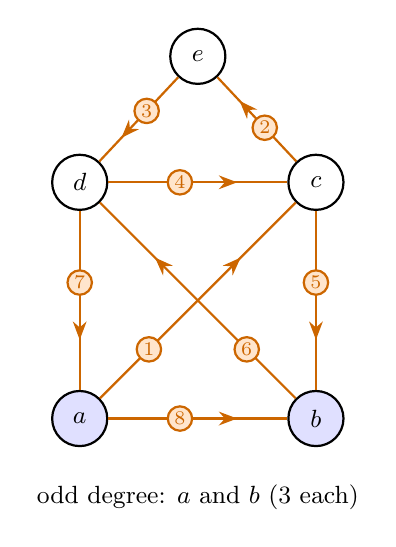
\begin{tikzpicture}[
  vertex/.style={circle, draw, thick, fill=white, minimum size=7mm, inner sep=0pt, font=\small},
  order/.style={circle, fill=orange!20, draw=orange!80!black, inner sep=1pt, font=\scriptsize},
  go/.style={thick, orange!80!black, postaction={decorate}, decoration={markings, mark=at position 0.72 with {\arrow{Stealth}}}},
]
  \node[vertex, fill=blue!12] (a) at (0,0) {$a$};
  \node[vertex, fill=blue!12] (b) at (3,0) {$b$};
  \node[vertex] (c) at (3,3) {$c$};
  \node[vertex] (d) at (0,3) {$d$};
  \node[vertex] (e) at (1.5,4.6) {$e$};
  % The path a, c, e, d, c, b, d, a, b uses all eight edges once.
  \foreach \u/\v/\n/\p in {a/c/1/0.25, c/e/2/0.4, e/d/3/0.4, d/c/4/0.4, c/b/5/0.4, b/d/6/0.25, d/a/7/0.4, a/b/8/0.4}
    \draw[go] (\u) -- node[order, pos=\p] {\n} (\v);
  \node[font=\small, align=center] at (1.5,-1) {odd degree: $a$ and $b$ (3 each)};
\end{tikzpicture}
